Let $f_{\theta^*}$ represent the trained neural network with an optimized set of parameters $\theta^*$. 
Then we can construct a prediction matrix $P = (f_{\theta^*}(t_d, a_v)) \in [0,1]^{{|D| \times |V|}}$  by collecting all predictions $f_{\theta^*}(t_d, a_v)$ from the trained neural network $f_{\theta^{*}}$ using the all pairs of data $(t_d,a_v) \in T \times A$ as illustrated in Figure \ref{fig:illutrate-preds}.

Upon the assumption that the trained neural network $f_{\theta^*}$ effectively encodes a shared understanding among legal experts of WTO agreements, our task is to find a set of directed edge weights $W^* = \{w^{*}_{ij} \mid w^{*}_{ij} = w^{*}(v_i, v_j) \text{ } s.t. \text{ } w^{*}(v_j, v_j) = 0 \text{ and } \sum_{v_i\in V}{w^{*}(v_i, v_j)} = 1 \text{ } \forall v_j \}$ %W^* = w(v_i, v_j)$ where
by exploiting the information encoded in the prediction matrix $P = (f_{\theta^*}(t_d, a_v)) \in [0,1]^{{|D| \times |V|}}$. This set of directed edge weights $W^{*} = \{w^{*}_{ij}\}$ shall represent a set of conditional praobability $P^{*}(v_j|v_i)$ how probably a source node $v_i$ clarifies the meaning of the target node $v_j$ compared to other source nodes
as closely as to a shared understanding of legal experts of WTO agreements.

To perform this task, this paper adopts a machine learning technique called \textit{Random Forest (RF)} that can rank input features, $\{f_{\theta^*}(t_d, a_{v_i}) \mid d \in D \text{ and } v_i \in V \setminus \{v_j\}\}$,  in terms of relative importance to explain the variance of output variables, $\{f_{\theta^*}(t_d, a_{v_j}) \mid d \in D \}$ for given target article $v_j \in V$. The step-by-step algorithm of \textit{Random Forest} will be explained in the next subsection.

% as illustrated in Figure \ref{fig:def-example}.
% This paper defines $W^*$ as a set of directed edge weights that best explains the co-citation pattern inside the prdiction matrix $P = (f_{\theta^*}(t_d, a_v)) \in [0,1]^{{|D| \times |V|}}$.  % that is visualized in Figure \ref{predidction_matrix}.

% To numerically ``best explains'' is that for given 


% == HEATMAP MATRIX == 
\begin{figure}[!tbp]
  \begin{subfigure}[b]{0.49\textwidth}
    \centering
    \resizebox{\columnwidth}{!}{
      \begin{tikzpicture}
        \foreach \i in {\xMin,...,5} {
            \draw [black] (\i,0) -- (\i,9) node [below] at (\i,4) {};
          }
        \foreach \i in {0,...,9} {
            \draw [black] (\xMin,\i) -- (5,\i) node [left] at (\xMin,\i) {};
          }
        \node [left] at (0,0.5) {\textbf{DS523}};
        \node [left] at (0,1.5) {\textbf{DS518}};
        \node [left] at (0,2.5) {\textbf{DS513}};
        \node [left] at (0,3.5) {\textbf{DS505}};
        % \node [left] at (0,4.5) {\textbf{DS4}};
        % \node [left] at (0,5.5) {\textbf{DS4}};
        \node [left] at (0,4.5) {\textbf{\vdots}};
        \node [left] at (0,5.5) {\textbf{DS31}};
        \node [left] at (0,6.5) {\textbf{DS22}};
        \node [left] at (0,7.5) {\textbf{DS18}};
        \node [left] at (0,8.5) {\textbf{DS2}};

        \node [left] at (4.8, 9.25) {\textbf{\ldots}};
        \node [left] at (3.8, 9.25) {\textbf{II:1}};
        \node [left] at (2.8, 9.25) {\textbf{II}};
        \node [left] at (1.85, 9.25) {\textbf{I:1}};
        \node [left] at (0.7,9.25) {\textbf{I}};

        \node [left] at (1.1,8.5) {\textbf{0.950}};
        \node [left] at (2.1,8.5) {\textbf{0.933}};
        \node [left] at (3.1,8.5) {\textbf{0.946}};
        \node [left] at (4.1,8.5) {\textbf{0.068}};

        \node [left] at (1.1,7.5) {\textbf{0.950}};
        \node [left] at (2.1,7.5) {\textbf{0.912}};
        \node [left] at (3.1,7.5) {\textbf{0.947}};
        \node [left] at (4.1,7.5) {\textbf{0.013}};

        \node [left] at (1.1,6.5) {\textbf{0.070}};
        \node [left] at (2.1,6.5) {\textbf{0.037}};
        \node [left] at (3.1,6.5) {\textbf{0.003}};
        \node [left] at (4.1,6.5) {\textbf{0.042}};

        \node [left] at (1.1,5.5) {\textbf{0.933}};
        \node [left] at (2.1,5.5) {\textbf{0.967}};
        \node [left] at (3.1,5.5) {\textbf{0.835}};
        \node [left] at (4.1,5.5) {\textbf{0.135}};

      \end{tikzpicture}
    }
    \label{fig:illutrate-preds}
    \caption{\textbf{Illustration of Prediction Matrix:} By defining row as a list of DS case numbers and column as legal articles, we can create $|D| \times |V|$ matrix that includes $f_{\theta^*}(t_d, a_v)$ for each cell.}
  \end{subfigure}
  \hfill
  \begin{subfigure}[b]{0.49\textwidth}
    \centering{
      \resizebox{\textwidth*\real{\heatmap}}{\textwidth*\real{\heatmap} * \real{1.7889}}{
        % This file was created by tikzplotlib v0.9.4.
\begin{tikzpicture}

\begin{axis}[
hide x axis,
hide y axis,
tick align=outside,
tick pos=left,
x grid style={white!69.0196078431373!black},
xmin=0, xmax=80,
xtick style={color=black},
y grid style={white!69.0196078431373!black},
ymin=0, ymax=143,
ytick style={color=black}
]
\addplot graphics [includegraphics cmd=\pgfimage,xmin=0, xmax=80, ymin=0, ymax=143] {pred_only.png};
\end{axis}

\end{tikzpicture}

      }
      \resizebox{\columnwidth}{!}{
        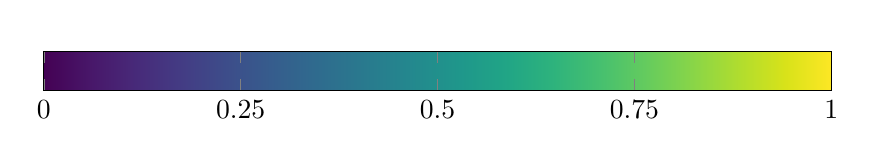
\begin{tikzpicture}
          \begin{axis}[
              hide axis,
              scale only axis,
              height=0pt,
              width=0pt,
              colormap/viridis,
              colorbar horizontal,
              point meta min=0,
              point meta max=1,
              colorbar style={
                  width=10cm,
                  height=0.5cm,
                  xtick={0,0.25,0.5,0.75,1}
                }]
            \addplot [draw=none] coordinates {(0,0)};
          \end{axis}
        \end{tikzpicture}
      }

      \caption{\textbf{Prediction Matrix:} This heatmap represents the $P$ from the actual data and its predictions from $f_{\theta^*}$}
      \label{predidction_matrix}
    }
  \end{subfigure}
  \caption{\textbf{Illustration of Prediction Matrix:} I collected all the predictions from the trained neural network $f_{\theta^*}$ and constructed prediction matrix $P$}
  \label{fig:illutrate-preds}
\end{figure}


% \[w : V \times V \to \Bbb R_{+} \text{ } s.t. \text{ } w(v_i, v_i) = 0 \text{ and } \sum_{v_i\in V}{w(v_i, v_j)} = 1 \text{  } \forall v_i, v_j \in V \] %\text{ and }\]
